%----------------------------------------------------------------------------------------
\begin{frame}
\begin{center}
\Huge{TOR - The Onion Router}
\end{center}
\end{frame}


%----------------------------------------------------------------------------------------
\begin{frame}
\frametitle{Présentation du réseau TOR}
Tor est un logiciel libre,
\begin{itemize}
\item grâce auquel existe le réseau d'anonymisation Tor
\item  soutenu par l'organisation The Tor Project.
\end{itemize}
$\Rightarrow$ Techniquement, Tor nous permet de se connecter à des machines sur Internet via des relais. 
\\$\Rightarrow$ Et cela de façon à ce qu'elles ne puissent pas identifier notre connexion (et donc de nous localiser).
\end{frame}


%----------------------------------------------------------------------------------------
\begin{frame}
\frametitle{A quoi sert TOR?}

Concrêtement, ça sert pour :
\begin{itemize}
\item  échapper au fichage publicitaire,
\item  publier des informations sous un pseudonyme,
\item  accéder à des informations en laissant moins de traces,
\item  déjouer des dispositifs de filtrage (dans sa fac, en Chine ou en Iran…),
\item  communiquer en déjouant des dispositifs de surveillances,
\item  tester son pare-feu,
\item  … et sûrement encore d'autres choses.
\end{itemize}
$\Rightarrow$ Tor dispose également d'un système de « services cachés » qui permet de fournir un service en cachant l'emplacement du serveur.
\end{frame}


%----------------------------------------------------------------------------------------
\begin{frame}
\frametitle{A quoi sert TOR?}

Tor est un réseau d'anonymisation, donc par définition, c'est difficile de faire un compte
précis.Tor ne fait rien pour cacher que nous utilisons Tor. Donc quand en utilisant
Tor, nous nous mettons au milieu de la foule des gens qui utilisent Tor. Plus
cette foule est grande, meilleur est l'anonymat.
\end{frame}

%----------------------------------------------------------------------------------------
\begin{frame}
\frametitle{Comment fonctionne Tor ?}
\begin{center}
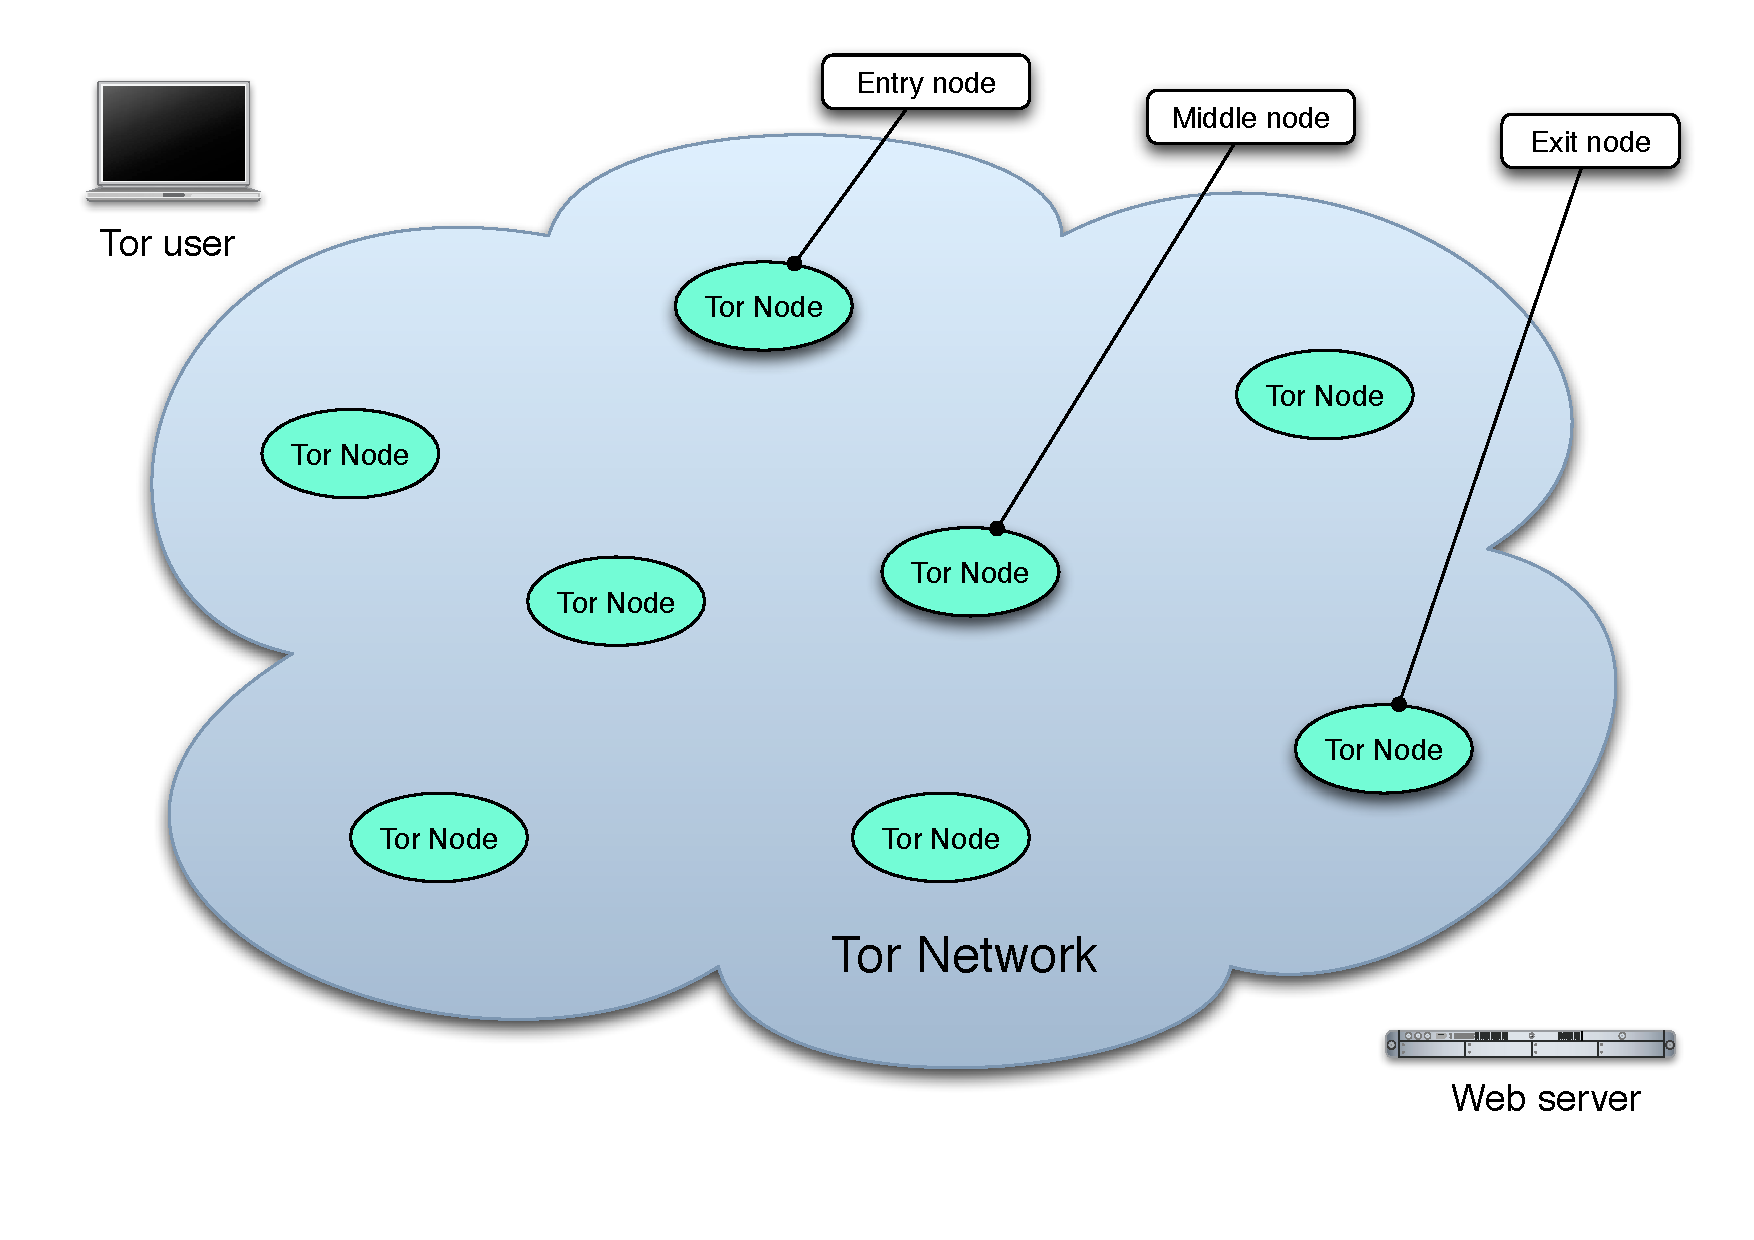
\includegraphics[keepaspectratio,width=\textwidth, height=.8\textheight]{./materials/tor-safe-selection}
\end{center}
\end{frame}


%----------------------------------------------------------------------------------------
\begin{frame}
\frametitle{Comment fonctionne Tor ?}
\begin{center}
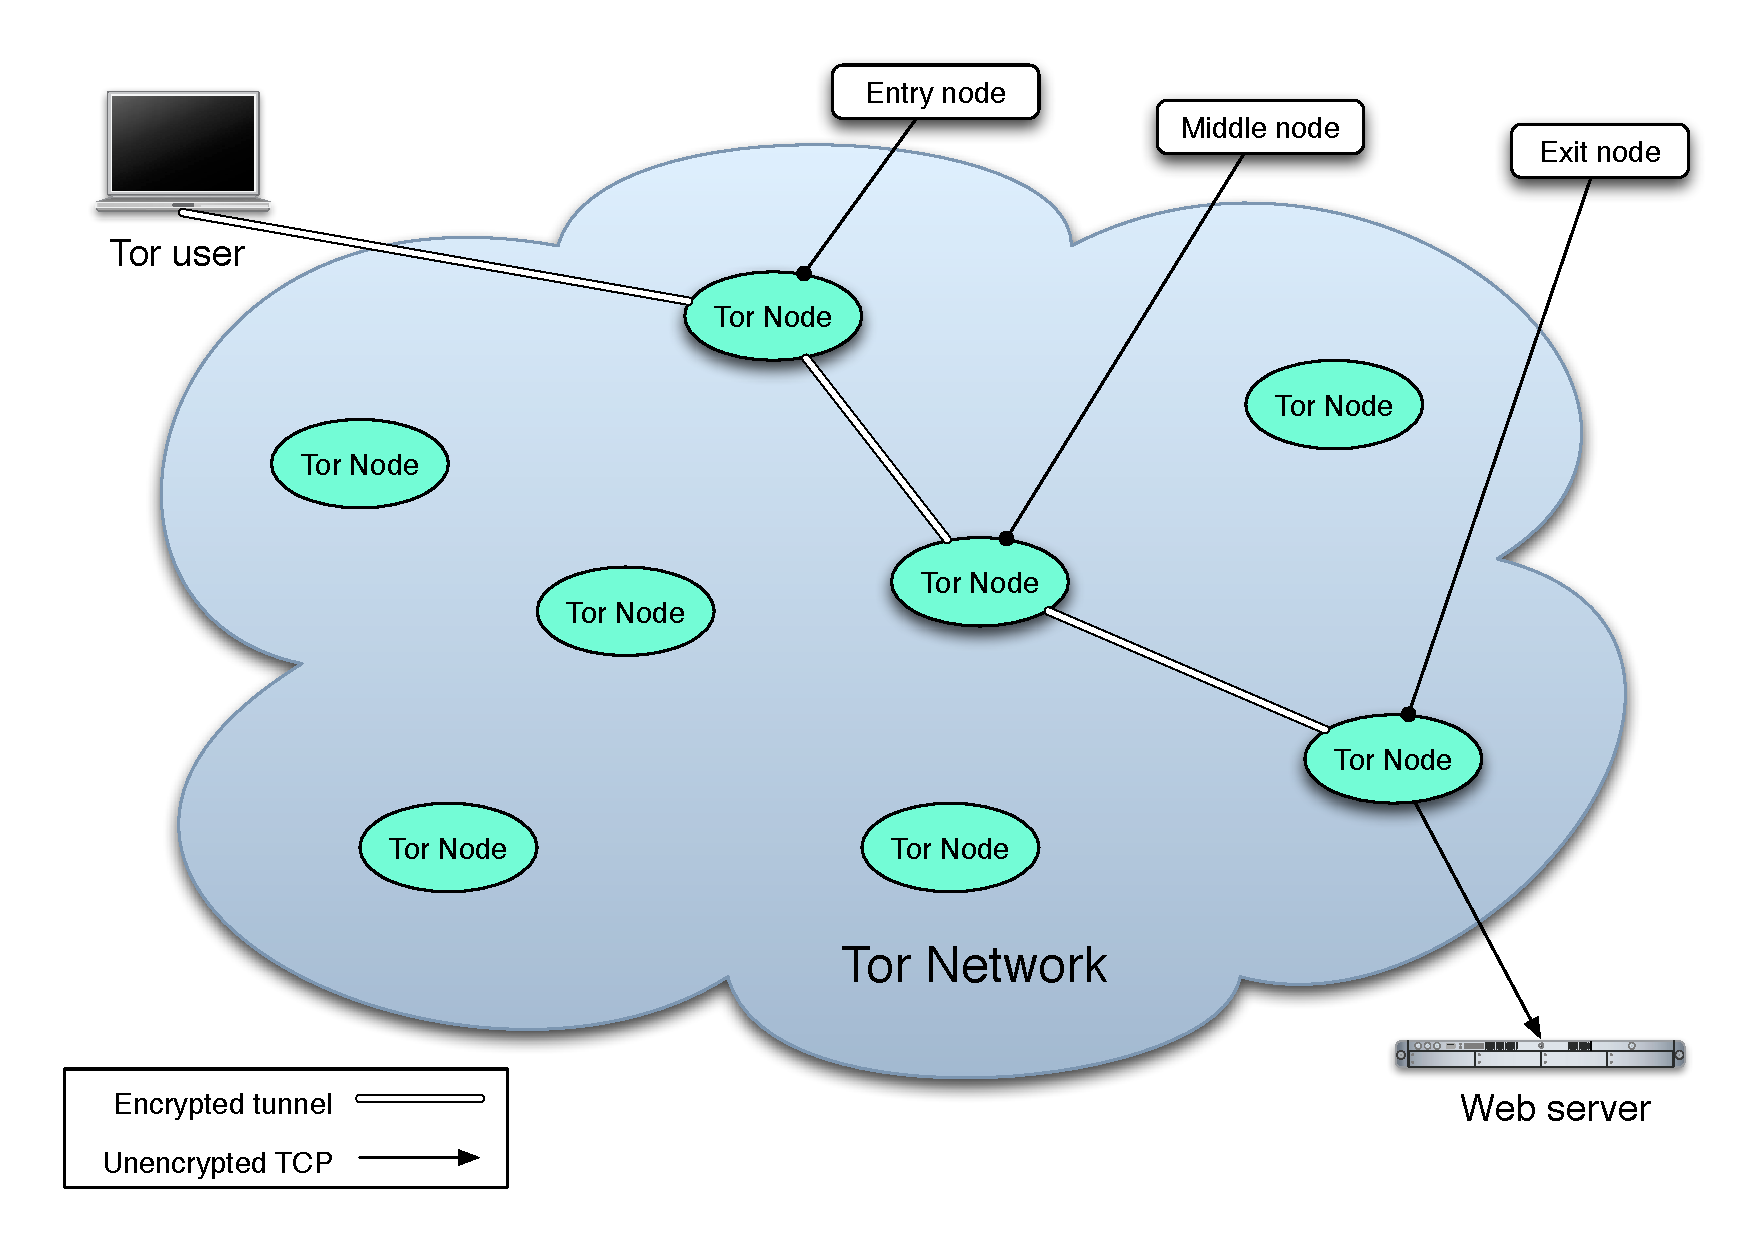
\includegraphics[keepaspectratio,width=\textwidth, height=.8\textheight]{./materials/tor-safe-path}
\end{center}
\end{frame}

%----------------------------------------------------------------------------------------
\begin{frame}
\frametitle{Comment fonctionne Tor ?}
\begin{center}
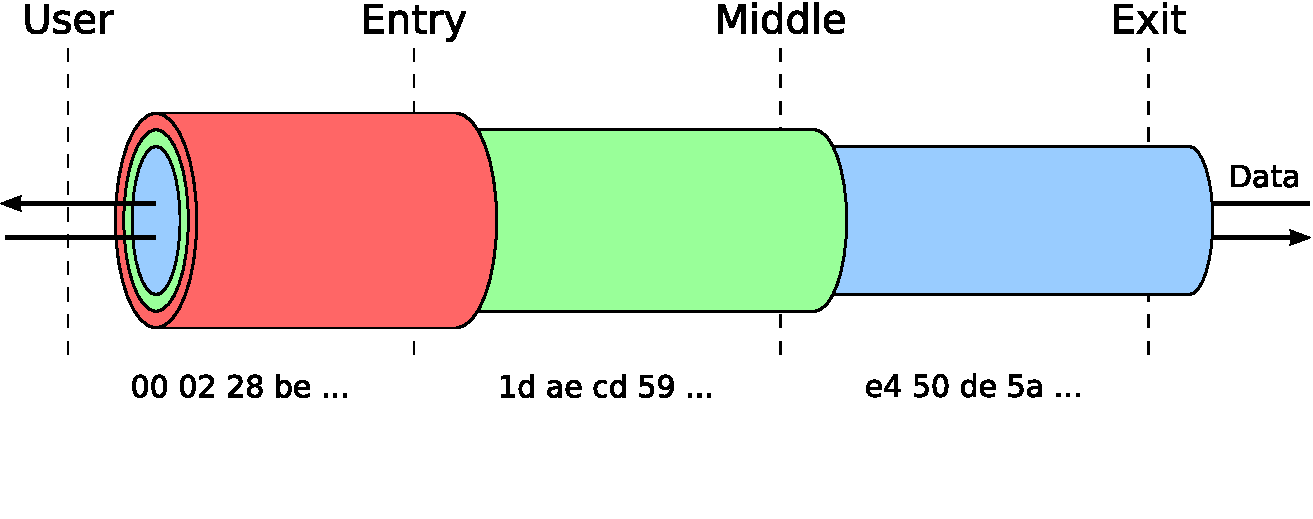
\includegraphics[keepaspectratio,width=\textwidth, height=.8\textheight]{./materials/tor-keys1}
\end{center}
\end{frame}

%----------------------------------------------------------------------------------------
\begin{frame}
\frametitle{Comment fonctionne Tor ?}

Ce tunnels se fait « en oignon » avec des couches de chiffrement empilées. Il y a une première
clé de chiffrement vers le nœud d'entrée, une second clé vers le nœud du milieu et
une dernière pour le nœud de sortie.
\\
Il faut noter que Tor ne s'occupe pas de chiffrer après le nœud de sortie. Comme n'importe
qui peut mettre en place un nœud de sortie, c'est une bonne idée de chiffrer sa communication
en plus (par exemple en se connectant aux sites web que l'on visite en HTTPS).
\\
Après, se déroule tout un processus pour établir un tunnel chiffré jusqu'au
nœud de sortie.
\end{frame}

%----------------------------------------------------------------------------------------
\begin{frame}
\frametitle{Utiliser Tor - Le Tor Browser}

Le Tor Browser est une version Extended Support de Firefox, auxquelles sont ajoutée les extensions préconfigurées permettant qu’au lancement du navigateur, celui-ci se connecte à Tor. 
\\$\Rightarrow$  Ainsi, toute la navigation qui se fait via ce navigateur est faite au travers du réseau Tor. 
\\$\Rightarrow$ C’est simplissime.

Toutes les versions (dans différentes langues, différents OS) sont disponibles sur le site du projet : https://www.torproject.org/projects/torbrowser.html
\end{frame}

%----------------------------------------------------------------------------------------
\begin{frame}
\frametitle{Le Tor Browser}
\begin{center}
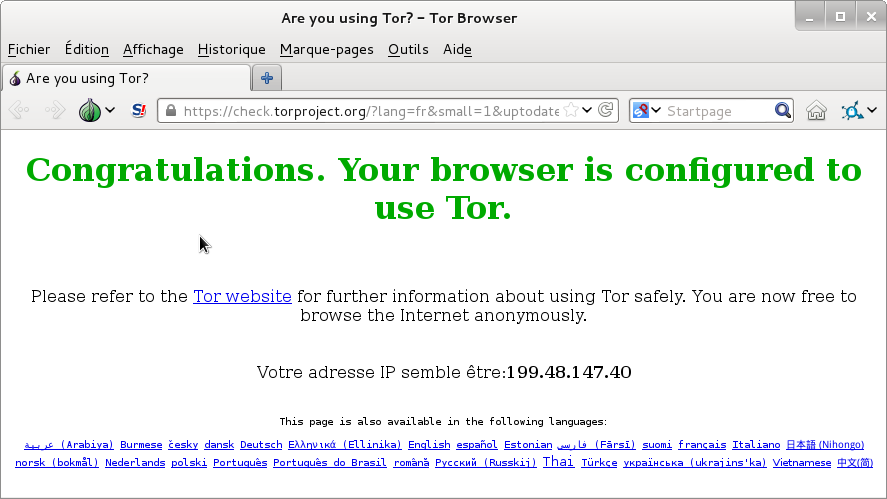
\includegraphics[keepaspectratio,width=\textwidth, height=.8\textheight]{./materials/tbb}
\end{center}
\end{frame}

%----------------------------------------------------------------------------------------
\begin{frame}
\frametitle{Tor Browser Launcher}
Pour avoir un Tor Browser toujours à jour, on peut installer le Tor Browser Launcher.
https://github.com/micahflee/torbrowser-launcher
\\
Il gère : 
\begin{itemize}
\item le téléchargement de la version la plus récente de TBB, dans votre langue et pour votre architecture
\item la mise à jour automatique (tout en conservant vos signets et préférences) manuel
\item la vérification de la signature GnuPG du TBB (pour être sûr de l’intégrité des fichiers)
\item ajoute un lanceur d’application "Tor Browser" dans le menu de votre environnement de bureau.
\end{itemize}
\end{frame}

%----------------------------------------------------------------------------------------
\begin{frame}
\frametitle{Utiliser Tor - Tails}

Tails est un système d'exploitation complet basé sur Linux et Debian, en live.
\begin{center}
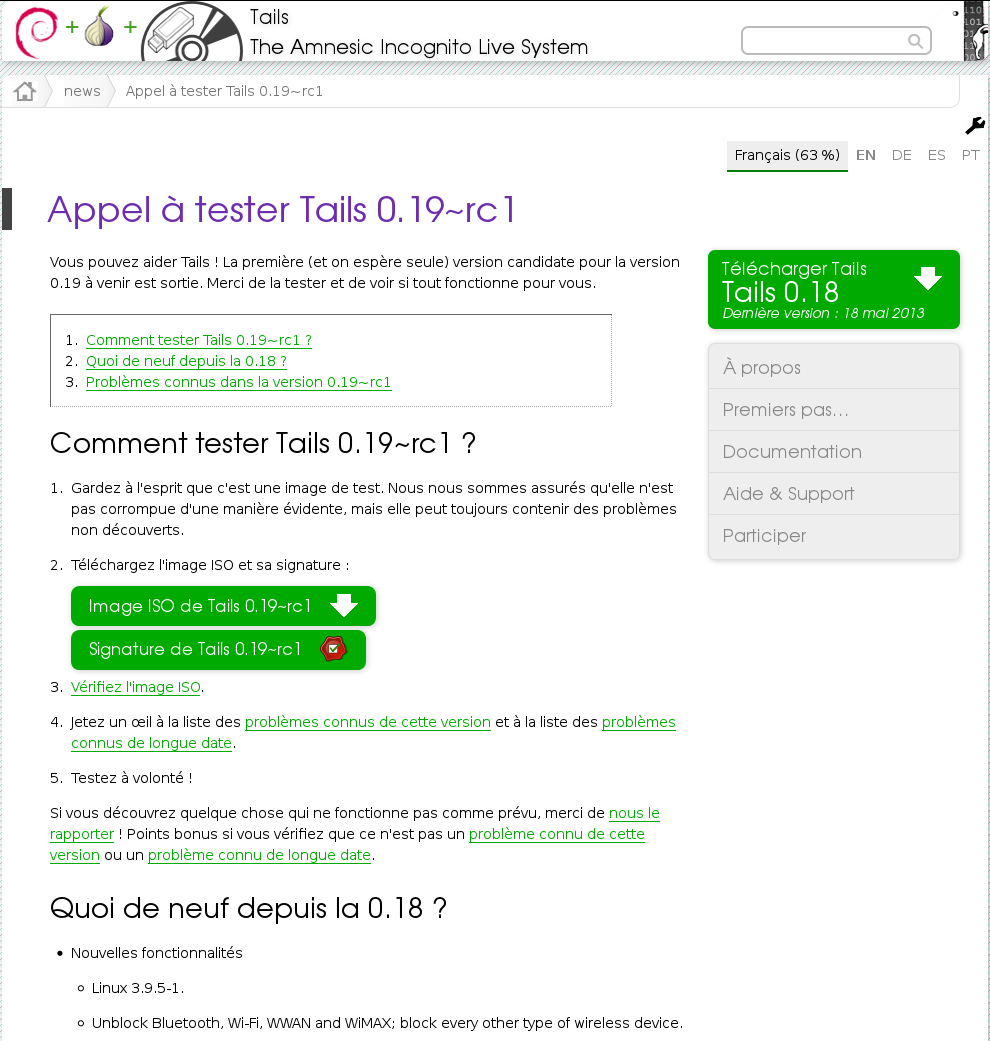
\includegraphics[keepaspectratio,width=\textwidth, height=.8\textheight]{./materials/tails}
\end{center}
\end{frame}

%----------------------------------------------------------------------------------------
\begin{frame}
\frametitle{Tor hidden service - les services cachés de TOR}

Tor permet aux clients et aux relais d’offrir des services cachés.Il est possible d'offrir un serveur web, un serveur SSH, etc, sans révéler son adresse IP aux utilisateurs.
\begin{itemize}
\item Tous ces sites ne sont accessibles que via le réseau Tor.
\item Ils portent une adresse qui se termine par .onion.
\item Des wikis et moteurs de recherches référencient ces services.
\end{itemize}
\end{frame}

%----------------------------------------------------------------------------------------
\begin{frame}
\frametitle{Soutenir Tor}

Il existe l'association NosOignons.net, qui propose des nœuds de sortie Tor financés par la communauté.
 https://nos-oignons.net
\begin{itemize}
\item En parler
\item Faire un don
\item Mettre en place un relais
\end{itemize}
\end{frame}


%----------------------------------------------------------------------------------------
\begin{frame}
\begin{center}
\Huge{Sur Internet, si c'est gratuit, c'est vous le produit }
\end{center}
\end{frame}


%----------------------------------------------------------------------------------------
\begin{frame}
\frametitle{Qu'est-ce que le pistage ?}


\begin{block}{Le pistage sur Internet}
\begin{itemize}
\justifying{
\item Le pistage est un terme qui comprend des méthodes aussi nombreuses et variées que les sites web, les annonceurs et d'autres utilisent pour connaître vos habitudes de navigation sur le Web. 
\item  Cela comprend des informations sur les sites que vous visitez, les choses que vous aimez, n'aimez pas et achetez. 
\item Ils utilisent souvent ces données pour afficher des pubs, des produits ou services spécialement ciblés pour vous. 
}
\end{itemize}
\end{block}
\end{frame}


%----------------------------------------------------------------------------------------
\begin{frame}
\frametitle{Comment est-on tracké?}

\justifying{
\begin{block}{Toutes les publicités nous espionnent}
\begin{itemize}
\item Le bouton Like de Facebook : il permet à FaceBook de savoir que vous avez visité ce site, même si vous n'avez pas cliqué sur ce bouton.
\item Même si vous vous êtes correctement déconnecté de Facebook.
\item De même pour le bouton le +1 de Google, les scripts de Google Analytics, 
\item Tous les publicité, Amazon...
\end{itemize}
\end{block}
}
\begin{center}

\includegraphics[scale=0.3] {./materials/Facebook_like.png}
\end{center}
\end{frame}


%----------------------------------------------------------------------------------------
\begin{frame}
\frametitle{L'extension Firefox LightBeam (ex Collusion)}
Cette extension permet de voir en temps réel qui nous traque et les interconnexions qu'a le site actuellement visité avec d'autres sites.
\begin{center}
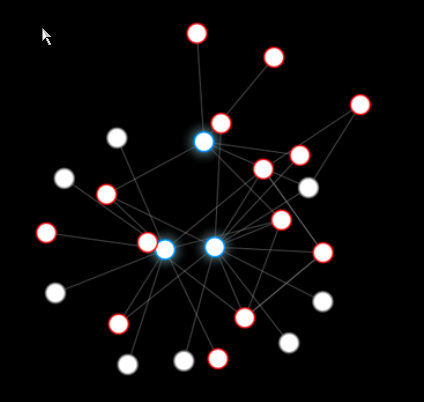
\includegraphics[scale=0.3] {./materials/Collusion.png}
\end{center}
\end{frame}

%----------------------------------------------------------------------------------------
\begin{frame}
\begin{center}
\Huge{Anomymat et extensions pour Firefox}
\end{center}
\end{frame}


%----------------------------------------------------------------------------------------
\begin{frame}
\frametitle{Noscript}

Bloque tous les trackers associés au site.

\begin{center}

\end{center}
\end{frame}


%----------------------------------------------------------------------------------------
\begin{frame}
\frametitle{Self destructing cookie}

Suppression automatisée des cookies

\begin{center}
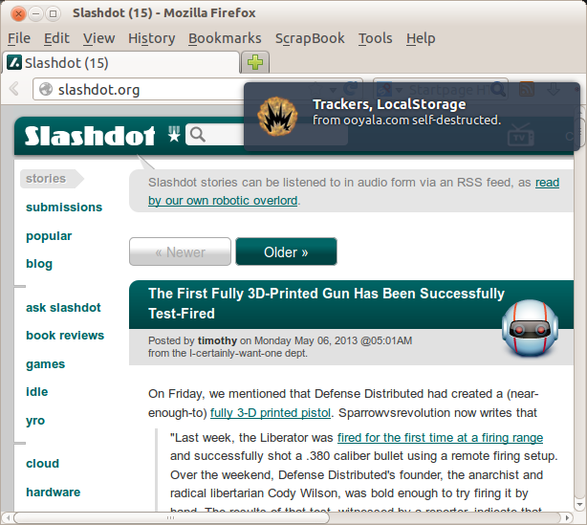
\includegraphics[scale=0.4] {./materials/selfdestructingcookie.png}
\end{center}
\end{frame}

%----------------------------------------------------------------------------------------
\begin{frame}
\begin{center}
\Huge{Changer de moteur de recherche}
\end{center}
\end{frame}

%----------------------------------------------------------------------------------------
\begin{frame}
\begin{center}
\frametitle{Duckduckgo - Google tracks you. We don't.}

\url{https://duckduckgo.com/}
\\

\includegraphics[scale=0.4] {./materials/DuckDuckGo.jpg}
\end{center}
\end{frame}

%----------------------------------------------------------------------------------------
\begin{frame}
\begin{center}
\Huge{Et pour plus de sécurité?}
\end{center}
\end{frame}

%----------------------------------------------------------------------------------------
\begin{frame}
\frametitle{HTTPSEverywhere}

Force le passage en https quand celui-ci est proposé par le site.

\begin{center}

\includegraphics[scale=0.4] {./materials/https-everywhere.jpg}
\end{center}

\end{frame}

%----------------------------------------------------------------------------------------
\begin{frame}
\frametitle{Certificate Patrol}
Permet de valider les certificats d'un site (lié à https).
\begin{center}
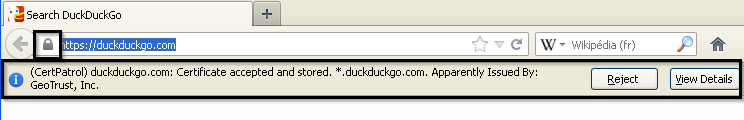
\includegraphics[scale=0.4] {./materials/CertificatePatrol.png}
\end{center}
\end{frame}

